\documentclass{homework}
% \usepackage{graphicx} % Required for inserting images
\usepackage{amsmath}
\usepackage{gensymb}
\usepackage{subfig}
\usepackage{float}

\class{ECEN 5738}
\title{Homework 3}
\author{Sean Jennings}
\date{February 19, 2023}

\begin{document}
\maketitle

\section{Problem 1}
\begin{letterenum}
\item
The sensitivity function $S(t) = dx/d\mu$ is given by:
\begin{equation*}
    \dot{S}(t) = A(t, \mu_0) S(t) + B(t, \mu_0)
\end{equation*}
where
\begin{equation*}
    A(t, \mu_0) = \frac{\delta}{\delta x} f(x(t, \mu); \mu) \eval_{\mu=\mu_0} \qquad
    B(t, \mu_0) = \frac{\delta}{\delta \mu} f(x(t, \mu); \mu) \eval_{\mu=\mu_0}.
\end{equation*}

Taking the jacobian w.r.t. $x$ and $\mu$ yields:
\begin{align*}
    \dot{S}(t) &= \mat{0 & -\mu \\ \mu & 0} \eval_{\mu=1} S(t) + \mat{
        -x_2(t, \mu_0) \\ x_1(t, \mu_0)
    } \\
    &= \mat{0 & -1 \\ 1 & 0} S(t) + \mat{
        -x_2(t, \mu_0) \\ x_1(t, \mu_0)
    }
\end{align*}

\item Figure \ref{fig:solution-sensitivity} shows the solution
to the sensitivity equation for the trajectory starting with initial
position $x(0) = [1, 0]^T$ and with parameter $\mu_0=1$.

\begin{center}
    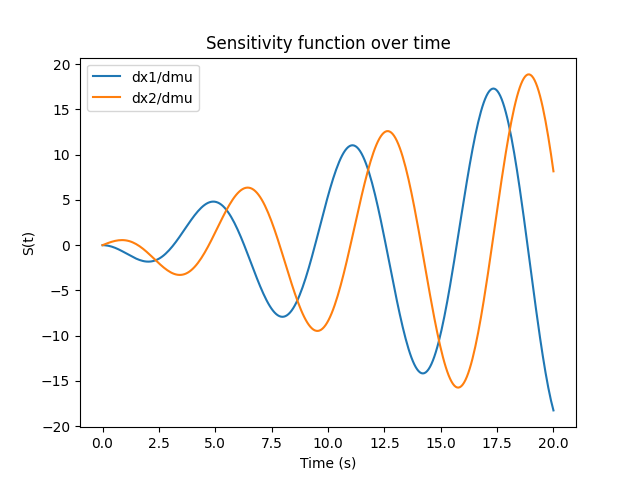
\includegraphics[width=0.8\linewidth]{Images/sensitivity.png}
    \captionof{figure}{Solution to sensitivity function}
    \label{fig:solution-sensitivity}
\end{center}

\item The solution for the sensitivity function shows that for a
given perturbation $\Delta \mu$ from the initial parameter $\mu_0$
the perturbation to the trajectory is oscillatory with an amplitude
the increases over time.

This makes sense since both the initial system as well as perturbations
are marginally stable. Changes in $\mu$ affect the frequency with
which the system completes a circular periodic orbit, and the trajectories
drift apart over time (for small perturbations).

\end{letterenum}

\section{Problem 2}

If $x_{eq}$ is an asymptotically stable equilibrium point, than
there exists an $r>0$ such that for all $x(0) \in B_r(x_{eq})$
the trajectory starting at $x(0)$ approaches $x_{eq}$ as $t$ approaches
infinity.

Then, any such $x\in B_r(x_{eq})$ (with $x \neq x_{eq}$) cannot be an
equilibrium point, since that would imply that a trajectory starting at $x$
would stay at $x$ and thus not approach $x_{eq}$. Therefore,
there exists a $\delta$ (equal to $r$) such that there are no
equilibrium points within $\delta$ of $x_{eq}$, and $x_{eq}$ is
an isolated equilibrium.

\section{Problem 3}
\begin{letterenum}
\item If we define $f: \R^2 \to \R^2$ to be the given dynamics function, then
we clearly see that $x_{eq} = [0, 0]^T$ has $f(x_{eq}) = 0$ and is therefore an
equilibrium point.

To linearize, we take the jacobian:
\begin{align*}
    \frac{\delta f}{\delta x} \eval_{x_{eq}} = \mat{
        a (3x_1^2 + x_2^2) & -1 + 2a x_1 x_2 \\
        1 + 2a x_1 x_2 & a (x_1^2 + 3 x_2^2) \\
    }\eval_{[x_1, x_2] = x_{eq}}  = \mat{
        0 & -1 \\
        1 & 0
    }.
\end{align*}
The linearized dynamics are then:
\begin{equation*}
    \dot{x} \approx f(x_{eq}) + \frac{\delta f}{\delta x} \eval_{x_{eq}} (x - x_{eq})
    = \mat{
        0 & -1 \\
        1 & 0
    } \mat{x_1 \\ x_2}
\end{equation*}

\item A phase portrait of the linearized dynamics is shown in figure
\ref{fig:linearized}.

\begin{center}
    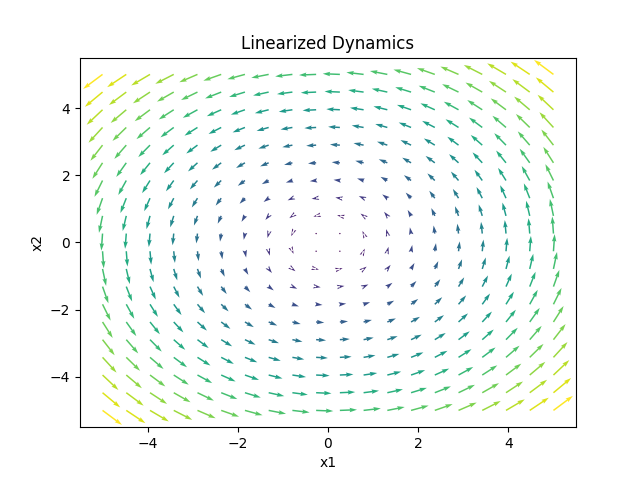
\includegraphics[width=0.8\linewidth]{Images/Linearized_Dynamics.png}
    \captionof{figure}{Phase Portrait of Linearized Dynamics}
    \label{fig:linearized}
\end{center}

\item In polar coordinates, we have:
\begin{align*}
    \frac{d}{dt}(r) &= \frac{d}{dt} (\sqrt{x_1^2 + x_2^2}) \\
        &= \frac{x_1 \dot{x}_1 + x_2 \dot{x}_2}{r} \\
        &= \frac{1}{r}\biggl(x_1 ( -x_2 + a x_1 r^2) + x_2(x_1 + x_2 r^2)\biggr) \\
        &= \frac{1}{r} (ar^2 ( x_1^2 + x_2^2)) = ar^3
\end{align*}

and
\begin{align*}
    \frac{d}{dt}(\theta) &= \frac{d}{dt} ( \tan^{-1}(x_2 / x_1)) \\
        &= \frac{x_1 \dot{x}_2 - x_2 \dot{x}_1}{x_1^2}
            \biggl(\frac{1}{1 + x_2^2/ x_1^2}\biggr) \\
        &= \frac{x_1 \dot{x}_2 - x_2 \dot{x}_1}{r^2} \\
        &= \frac{x_1(x_1 + ax_2r^2) - x_2(-x_2 + a x_1r^2)}{r^2} \\
        &= \frac{x_1^2 + x_2^2}{r^2} = 1.
\end{align*}
A phase portrait for the nonlinear dynamics is shown in figure \ref{fig:nonlinear}.

\begin{center}
    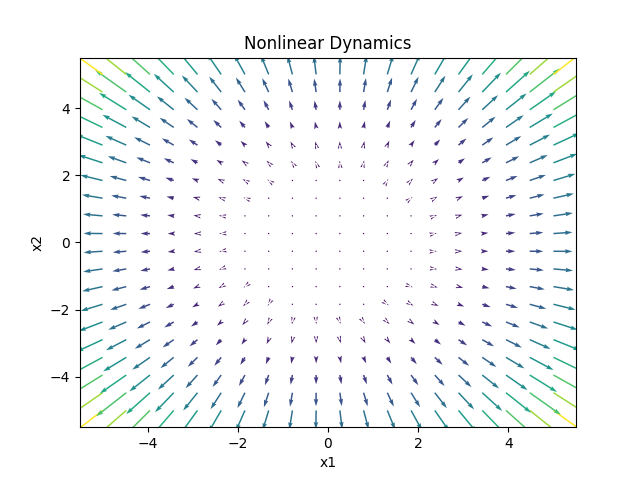
\includegraphics[width=0.8\linewidth]{Images/Nonlinear_Dynamics.png}
    \captionof{figure}{Phase Portrait of Nonlinear Dynamics}
    \label{fig:nonlinear}
\end{center}


\item Qualitatively, the phase portrait for the nonlinear dynamics overall
points away from the origin, as governed by the nonlinear $\dot{r} = ar^3$
component. If we zoom in on the origin, as seen in figure \ref{fig:nonlinear-zoomed},
we can see that the phase portrait again appears to resemble the linearized dynamics
of figure \ref{fig:linearized}. Unfortunately for the stability of this system,
the nonlinear $r^3$ term, will (at first slowly) push the state out of the
circular periodic orbits of the linearized system, eventually reaching
states where the linearization is no longer a good approximation.

\begin{center}
    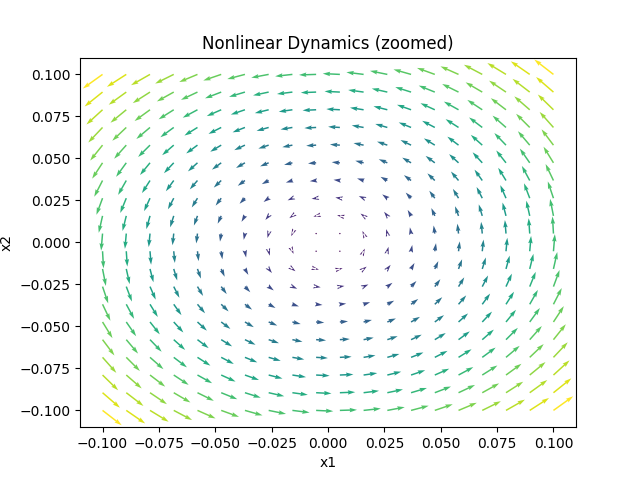
\includegraphics[width=0.8\linewidth]{Images/Nonlinear_Dynamics_(zoomed).png}
    \captionof{figure}{Phase Portrait of Nonlinear Dynamics (zoomed)}
    \label{fig:nonlinear-zoomed}
\end{center}
\end{letterenum}

\section{Problem 4}
\begin{letterenum}
\item Since each $(p_i(x))^2$ is nonnegative, the sum $\sum_{i=1}^m (p_i(x))^2$
 also is.

\item Using the fact that a matrix $A$ with non-negative eigenvalues can
be written as the product of upper triangular matrices $A = R^T R$, we have:
\begin{equation*}
    V(x) = \mat{x^3 & x^2 & x & 1} R^T R \mat{x^3 \\ x^2 \\ x \\ 1} 
        = p(x)^T p(x)
        = \sum_{i=1}^{4} (p_i(x))^2
\end{equation*}
where we have defined $p: \R \to \R^4$ to be $p(x) = R [x^3, x^2, x, 1]^T$.
Each entry $p_i$ of $p$ is a polynomial with degree 3, and we see that $V(x)$ is
a sum of squares and thus nonnegative.

\end{letterenum}



\end{document}
